\documentclass[11pt,a4paper]{article}

\usepackage[T1]{fontenc}
\usepackage[utf8]{inputenc}
\usepackage{lmodern}
\usepackage{microtype}
\usepackage{amsmath,amssymb,amsthm,mathtools}
\usepackage{booktabs}
\usepackage{enumitem}
\usepackage{graphicx}
\usepackage{hyperref}

\newtheorem{theorem}{Theorem}[section]
\newtheorem{proposition}[theorem]{Proposition}
\newtheorem{lemma}[theorem]{Lemma}
\newtheorem{conjecture}[theorem]{Conjecture}
\theoremstyle{definition}
\newtheorem{definition}[theorem]{Definition}
\newtheorem{question}[theorem]{Research Question}

\newcommand{\True}{\mathbf{T}}
\newcommand{\False}{\mathbf{F}}
\newcommand{\Both}{\mathbf{B}}
\newcommand{\Neither}{\mathbf{N}}
\newcommand{\pos}[1]{+\!#1}
\newcommand{\neginfo}[1]{-\!#1}
\newcommand{\FDE}{\mathrm{FDE}}
\newcommand{\MCp}{\mathrm{MC}^{+}}
\newcommand{\MCm}{\mathrm{MC}^{-}}
\newcommand{\Rp}{R^{+}}
\newcommand{\Rm}{R^{-}_{\mathrm{nec}}}
\newcommand{\llbracket}{\mathopen{[\![}}
\newcommand{\rrbracket}{\mathclose{]\!]}}
\newcommand{\statusestablished}{\textsc{Status: established at the semantic level.}}
\newcommand{\statusopen}{\textsc{Status: open.}}
\newcommand{\statusconjectural}{\textsc{Status: conjectural.}}

\title{Decomposing Modal Collapse:\\A Four-Valued Analysis of G\"odel--Scott Positivity}
\author{Julian Voigt}
\date{Working manuscript, version 0.19}

\begin{document}
\maketitle

\begin{abstract}
I study the inferential architecture of the G\"odel--Scott ontological theory under a bilateral four-valued semantics admitting both inconsistent and incomplete information. Scott's classical theory is fixed as a control system and reconstructed incrementally over a Belnap--Dunn/FDE propositional kernel, bilateral Kripke modality, actualist individual quantification, and higher-order property quantification. The original conjecture that positive and negative modal collapse might separate is falsified under involutive FDE negation: the informative signed collapse schemata are equivalent by substitution. The substantive decomposition instead occurs upstream. Scott's A1 splits into directional information flows with distinct roles, mere positive support is insufficient for the T1 analogue, and two explicit S5 models show that natural bilateral essence does not make support-based Godlikeness an essence automatically: positive T2 fails through separate glut and gap mechanisms. A relevant consistency/completeness package recovers T2, and Lean 4.30.0 machine-checks the implication. Gate 8 then compares alternative architectures. Once Scott T2 is available, symmetry alone suffices for positive T3, while a non-symmetric S4 model refutes the corresponding replacement. Project-internal exact positive Godlikeness internalizes local reflection, and a literature-grounded bilateral Anderson candidate admits positive necessary Godlike existence without positive modal collapse. The Fitting comparison reveals a further structural boundary. A naive unrestricted bilateral extension domain makes the relevant Fitting consistency package incompatible with any positive Godlike witness; Lean proves this comprehension obstruction directly. I therefore reconstruct the substantive Fitting candidate over a selected FDE-negation-closed domain of admissible extensions, without globally excluding gluts. In that non-vacuous setting, the extensional Godlikeness-as-essence theorem requires no positivity-rigidity premise, the de-re possibility-to-necessity route requires no frame condition, and de-dicto lifting requires only stability of the positive Godlikeness extension rather than full bilateral extension stability. The classification-based Fitting recovery package can be weakened so that exemplification consistency is required only on the negatively classified branch of the A1-L proof; restoring A1-R reconstructs the stronger consistency condition. A second recovery route bypasses positivity completeness entirely. I derive its Godlike-indiscernibility premise from a quotient-style saturation principle on positive-property profiles. Negation closure upgrades this to bilateral factorization, and quotient-respecting extensions are closed under the basic FDE operations, while a finite countermodel shows that ordinary FDE algebra closure alone does not generate the quotient. The same failure persists after adding A2-style positivity monotonicity and even full domain-level entailment closure. Indeed, Lean shows that naively closing an admissible domain containing FDE bottom under arbitrary global entailment forces unrestricted bilateral comprehension and recreates the Godlike-witness obstruction under relevant consistency. The quotient admits a more canonical formulation instead: profile saturation is the fixed-point condition of an extensive, monotone, idempotent closure operator giving the least quotient-respecting extension above any bilateral extension. Lean now constructs the entity quotient explicitly, proves bilateral extension push/pull round trips, characterizes profile-compatible actual existence exactly as factorization through accessible source quotients, and proves quotient actualist entailment equivalent to ordinary entailment on pullbacks. A split-existence finite model shows why factorization matters, while exhaustive bounded comparisons retain genuine glut and gap values. By contrast, an ultrafilter-style complement-decision principle with relevant consistency or A1-R reconstructs the earlier classification route. Finite witnesses also separate positive-only extension stability from its stronger bilateral predecessor. A new rigidity bridge shows that forward admissible positivity transport derives backward positive Godlikeness reflection, while converse positivity transport along existing edges derives forward persistence without requiring frame symmetry. Symmetry plus forward rigidity entails this converse transport, but 32 asymmetric finite models satisfy both transport directions, showing that accessibility symmetry is stronger than the de-dicto proof needs. A complete-S5 Fitting model has positive necessary Godlike existence, genuine inconsistent extension information, and failure of positive modal collapse. The remaining questions concern four-valued filter structure on the quotient fixed points, further G-triggered restriction of converse positivity transport, and generalization beyond relational control semantics.
Gate 10 places a first algebraic constraint on that open direction. On the quotient extension algebra, Lean proves that point evaluation is a proper prime FDE truth-order filter which designates gluts but leaves gaps complement-undecided. An exhaustive two-point audit confirms that ordinary, prime, and non-adjunctive two-filters survive without automatic complement decision, and supplies a non-vacuous ordinary-filter model where local positivity completeness fails.
Gate 11 discharges the deferred modal representation task. Lean now defines paired universal/core and hit/witness neighborhoods, proves bilateral box/diamond duality, embeds every Kripke frame exactly at all four signed modal clauses, and derives classical modal recovery from complement duality. The exhaustive two-world local audit separates four principal relational pairs from twelve additional non-principal complement-dual pairs; arbitrary non-dual pairs can produce either gluts or gaps from classically valued inputs.
\end{abstract}

\section{Introduction}
\label{sec:introduction}

G\"odel's ontological argument and Dana Scott's well-known modification form an unusually compact laboratory for higher-order modal reasoning. Their interest for the present paper is structural rather than theological. The theory combines a primitive predicate of positive properties, modal rigidity, higher-order quantification, essence, and necessary existence, while its derivational behavior has been studied extensively with automated and interactive theorem provers \cite{BenzmuellerScott2025,BenzmuellerFuenmayor2019}. In Scott's variant the main existence theorem is accompanied by the well-known phenomenon of \emph{modal collapse}, schematically
\[
  \chi \rightarrow \Box\chi,
\]
according to which every truth is necessary.

Recent machine-checked work sharpens the diagnosis of this phenomenon. In particular, the existence of an ultrafilter-like structure among positive properties does not by itself force collapse; rigidity of positivity is a principal modal ingredient \cite{Benzmueller2026Collapse}. This raises a natural question that classical two-valued semantics cannot express: which information flows inside positivity, essence, and necessary existence are actually responsible for reconstructing the collapse mechanism?

I study this question in a bilateral four-valued setting. Instead of assigning a single Boolean value to a formula, I track positive and negative support independently. A formula may therefore be supported only, opposed only, both supported and opposed, or neither. This gives the four values
\[
  \True=(1,0),\qquad
  \False=(0,1),\qquad
  \Both=(1,1),\qquad
  \Neither=(0,0),
\]
following the Belnap--Dunn/FDE tradition \cite{Belnap1977,Dunn1976}.

The central research question is:

\begin{question}[Upstream structure of modal collapse]
Under a four-valued bilateral modal semantics, which components of positivity-negation transfer, positivity rigidity, informational regularity, essence, and higher-order witness structure reconstruct the classical G\"odel--Scott modal-collapse mechanism?
\end{question}

The informative signed collapse pair is
\[
  \MCp:\quad \pos{\chi}\Rightarrow\pos{\Box\chi},
  \qquad
  \MCm:\quad \neginfo{\chi}\Rightarrow\pos{\Box\neg\chi}.
\]
These are not independent in the fixed FDE setting. Since \(\neginfo{\chi}\) is equivalent to \(\pos{\neg\chi}\), \(\MCm\) is exactly \(\MCp\) instantiated at \(\neg\chi\), and conversely by involutive negation. The original collapse-separation conjecture is therefore falsified rather than preserved by an ad hoc semantic modification.

The decomposition instead occurs upstream. Scott's A1 splits into two independent directional information flows,
\[
  A1_L:\quad \neginfo{P(\varphi)}\Rightarrow\pos{P(\neg\varphi)},
\]
\[
  A1_R:\quad \pos{P(\neg\varphi)}\Rightarrow\neginfo{P(\varphi)}.
\]
The two directions acquire different jobs. \(A1_R\), together with a semantic positive-support form of A2, yields possible exemplification for truth-only positive properties. \(A1_L\) participates in the reflection and essence branch. A positivity glut blocks the unrestricted T1 analogue because the negative support produced by the classical reductio may already be present.

Gate 6 pushes this upstream diagnosis further. A natural bilateral reconstruction of Scott's essence definition does not make Godlikeness an essence automatically. Two finite S5 models satisfy the earlier control axioms, strong A1, and positive rigidity while refuting positive T2: one fails through inconsistent exemplification and one through incomplete positivity information. A targeted regularity package recovers positive T2, after which the necessary-existence branch becomes comparatively robust. Positive support for A5 suffices for a positive T3 in S5, even if necessary existence itself is glutty.

Once positive T2 and T3 are available, modal collapse follows directly from essence and constant-property embedding. The central non-classical difficulty is therefore no longer modal collapse itself, nor even T3. It is the weakest principled recovery of Godlikeness-as-essence from the lower-level four-valued Scott machinery.

The contribution sought is not a ``stronger proof of God''. The intended contribution is an explanatory dependency analysis showing where four-valued inconsistency and incompleteness alter the inferential architecture of the Scott theory, including negative results and countermodels that locate hidden classical regularity assumptions.

\paragraph{Methodological discipline.}
The development proceeds conservatively. I freeze a classical Scott baseline, fix the propositional and modal semantics, and then lift individual G\"odel--Scott principles only when their semantic prerequisites are explicit. Failed conjectures are retained as results rather than repaired by changing the semantics after the fact. Implication-sensitive clauses are represented by signed semantic entailment relations rather than by prematurely choosing a four-valued object-language conditional.

\paragraph{Status of this manuscript.}
Version 0.6 reports Gates 0--6: the classical baseline; propositional, modal, and positivity semantics; the collapse and reflection analyses; the A2/T1/A3/Godlikeness reconstruction; bilateral essence and necessary existence; finite glut/gap countermodels to positive T2; a sufficient T2 recovery theorem; conditional positive T3; discharge of the global witness interface; and the essence-compressed modal-collapse theorem. The next phase is mechanization and semantic-minimality analysis centered on T2.

\section{Classical Scott Baseline}
\label{sec:scott}

\statusestablished

I use Scott's variant as the classical control theory, following the modern formal presentation of Benzm\"uller and Scott \cite{BenzmuellerScott2025}. The reference environment uses intensional properties over possible worlds, actualist quantification over individuals, possibilist quantification over properties, and an S5 reference frame. Later experiments may weaken the modal frame, but such changes are not part of the baseline.

Let \(P(\varphi)\) mean that property \(\varphi\) is positive. The relevant axioms and definitions are:

\begin{align}
\mathrm{A1}\quad & \neg P(\varphi) \leftrightarrow P(\neg\varphi),\\
\mathrm{A2}\quad & P(\varphi)\land \Box\forall^E y\,(\varphi(y)\rightarrow\psi(y))\rightarrow P(\psi),\\
\mathrm{D1}\quad & G(x) \equiv \forall\varphi\,(P(\varphi)\rightarrow\varphi(x)),\\
\mathrm{A3}\quad & P(G),\\
\mathrm{A4}\quad & P(\varphi)\rightarrow\Box P(\varphi),\\
\mathrm{D2}\quad & \varphi\operatorname{Ess}x \equiv \varphi(x)\land
  \forall\psi\bigl(\psi(x)\rightarrow\Box\forall^E y(\varphi(y)\rightarrow\psi(y))\bigr),\\
\mathrm{D3}\quad & NE(x) \equiv \forall\varphi\bigl(\varphi\operatorname{Ess}x\rightarrow
  \Box\exists^E y\,\varphi(y)\bigr),\\
\mathrm{A5}\quad & P(NE).
\end{align}

The standard theorem chain includes
\begin{align}
\mathrm{T1}\quad & P(\varphi)\rightarrow\Diamond\exists^E x\,\varphi(x),\\
& \Diamond\exists^E x\,G(x),\\
\mathrm{T2}\quad & G(x)\rightarrow G\operatorname{Ess}x,\\
\mathrm{T3}\quad & \Box\exists^E x\,G(x),\\
\mathrm{MC}\quad & \chi\rightarrow\Box\chi.
\end{align}

For the present project, T3 is a control theorem while MC is the main structural target. A proposed four-valued theory must state precisely in what sense this classical system is recovered when all relevant valuations are restricted to the consistent and complete values \(\True\) and \(\False\).

The project-level baseline, including quantifier conventions and dependency notes, is maintained in \texttt{docs/SCOTT\_BASELINE.md}.

\section{Four-Valued Propositional Kernel}
\label{sec:kernel}

\statusestablished

The propositional base follows the information structure of Belnap--Dunn First-Degree Entailment \cite{Belnap1977,Dunn1976}. Every formula \(\varphi\) receives two independent bits
\[
  v(\varphi)=(t(\varphi),f(\varphi))\in\{0,1\}^2,
\]
where \(t(\varphi)=1\) represents positive support and \(f(\varphi)=1\) negative support. I write \(\pos{\varphi}\) and \(\neginfo{\varphi}\) for these two satisfaction conditions.

\begin{center}
\begin{tabular}{ccc}
\toprule
Value & Pair & Reading \\
\midrule
\(\True\) & \((1,0)\) & positive support only \\
\(\False\) & \((0,1)\) & negative support only \\
\(\Both\) & \((1,1)\) & both positive and negative support \\
\(\Neither\) & \((0,0)\) & neither positive nor negative support \\
\bottomrule
\end{tabular}
\end{center}

Atoms receive positive and negative support independently. The connectives are fixed by the bilateral clauses
\begin{align*}
\pos{\neg\varphi} &\iff \neginfo{\varphi}, &
\neginfo{\neg\varphi} &\iff \pos{\varphi},\\
\pos{(\varphi\land\psi)} &\iff \pos{\varphi}\land\pos{\psi}, &
\neginfo{(\varphi\land\psi)} &\iff \neginfo{\varphi}\lor\neginfo{\psi},\\
\pos{(\varphi\lor\psi)} &\iff \pos{\varphi}\lor\pos{\psi}, &
\neginfo{(\varphi\lor\psi)} &\iff \neginfo{\varphi}\land\neginfo{\psi}.
\end{align*}

Positive semantic consequence preserves positive satisfaction:
\[
  \Gamma\models_{\FDE}\varphi
\]
iff every valuation positively satisfying every member of \(\Gamma\) also positively satisfies \(\varphi\). Equivalently, the positively designated values are \(\{\True,\Both\}\). Negative satisfaction remains separately observable and will be used for bilateral meta-conditions in later sections.

Crucially, no object-language implication is fixed at this stage. Although \(\neg\varphi\lor\psi\) is definable, treating it as \emph{the} conditional would prematurely determine the lifting of A2, D1, D2, and D3.

\begin{proposition}[Paraconsistency]
The kernel is non-explosive: \(p,\neg p\not\models_{\FDE}q\).
\end{proposition}
\begin{proof}
Let \(v(p)=\Both\) and \(v(q)=\Neither\). Then \(p\) and \(\neg p\) are both positively satisfied, while \(q\) is not.
\end{proof}

\begin{proposition}[Paracompleteness]
Excluded middle is not valid: \(\not\models_{\FDE}p\lor\neg p\).
\end{proposition}
\begin{proof}
Let \(v(p)=\Neither\). Negation preserves \(\Neither\), so neither disjunct is positively satisfied and hence neither is their disjunction.
\end{proof}

\begin{proposition}[Classical recovery of the propositional fragment]
If atomic valuations are restricted to \(\{\True,\False\}\), then the clauses for \(\neg\), \(\land\), and \(\lor\) remain inside \(\{\True,\False\}\) and coincide with the classical truth tables.
\end{proposition}
\begin{proof}
Immediate by structural induction on formulas using the bilateral clauses above.
\end{proof}

The full gate specification is maintained in \texttt{docs/FOUR\_VALUED\_KERNEL.md}.

\section{Four-Valued Modal Semantics}
\label{sec:modal}

\statusopen

This section is the dependency of Gate 2 and is intentionally not frozen in version 0.1. The first conservative candidate is a relational bilateral Kripke semantics in which
\[
  w\models^{+}\Box\varphi
  \quad\text{iff}\quad
  \forall v\,(wRv\Rightarrow v\models^{+}\varphi),
\]
and
\[
  w\models^{-}\Box\varphi
  \quad\text{iff}\quad
  \exists v\,(wRv\land v\models^{-}\varphi).
\]
A corresponding treatment of \(\Diamond\) must be stated independently rather than assumed by classical duality.

The relational candidate will be compared with a neighborhood-style formulation before either is adopted as the project semantics. Four-valued modal logics with Belnapian truth values already have substantial semantic and proof-theoretic literature \cite{OdintsovWansing2010,RivieccioJungJansana2017}, and recent work develops an S5-based four-valued treatment of essence and accident modalities \cite{Petrukhin2026}. The purpose of Gate 2 is therefore not to reinvent four-valued modality, but to determine which established or conservative modal lift best exposes the later G\"odel--Scott decomposition.

\begin{question}
Under what conditions does the modal lift recover classical \(\Box\) and \(\Diamond\) on the \(\{\True,\False\}\) fragment?
\end{question}

\begin{question}
Which dualities between necessity, possibility, and negation survive in the presence of \(\Both\) and \(\Neither\)?
\end{question}

\section{Bilateral Positivity}
\label{sec:positivity}

\statusestablished

The positivity predicate \(P\) is the central non-logical primitive of the Scott theory. In the four-valued reconstruction, statements of the form \(P(\varphi)\) carry positive and negative information independently.

\subsection{The property domain}
\label{sec:property-domain}

Scott's D1, D2, and D3 quantify over properties, so the reconstruction must say what the property domain is before those definitions can be lifted. I deliberately do not fix it as a powerset, as a set of intensional functions, or by any comprehension principle. The Scott branch instead treats properties as an arbitrary type \(\Pi\) equipped with

\begin{itemize}
  \item signed exemplification relations \(\mathrm{ex}^{+},\mathrm{ex}^{-}\subseteq W\times D\times\Pi\);
  \item signed positivity predicates \(P^{+},P^{-}\subseteq W\times\Pi\);
  \item a property-negation operation \(\nu:\Pi\to\Pi\);
  \item a distinguished element \(G\in\Pi\).
\end{itemize}

Nothing forces \(\Pi\) to be closed under any operation beyond \(\nu\), and no instance of \(\Pi\) is privileged. Every theorem below is therefore a statement about all such structures. This is also what makes the finite countermodels legitimate rather than approximate: a model whose property domain is the four-element set \(\{G,\nu G,Z,\nu Z\}\) is an instance of the semantics, not a truncation of an intended larger one.

The reading of \(\nu\) as \emph{negation} is likewise not built in. It is constrained only by whatever is assumed explicitly, principally
\[
  \mathrm{ex}^{+}(w,x,\nu\varphi)\iff\mathrm{ex}^{-}(w,x,\varphi)
\]
together with the directional A1 conditions below. In particular, involutivity
\[
  \nu\nu\varphi=\varphi
\]
is a further assumption rather than part of the signature. The mechanized \(T1_T\) and \(T2^+\) theorems do not use it. The substitution arguments in the remainder of this section, and the rigidity-coupling proposition in Section~\ref{sec:collapse}, do use it; I flag this explicitly at each point rather than treating property negation as if it were the object-language connective of Section~\ref{sec:kernel}.

The Fitting comparison in Section~\ref{sec:fitting-obstruction} differs from the Scott branch precisely here. It replaces this abstract domain by a typed intension/extension architecture in which properties have internal structure, and the resulting freedom to choose which extensions are admissible is what generates the obstruction and the repair analyzed there.

\subsection{Directional decomposition of A1}

Scott's A1 is
\[
  \neg P(\varphi)\leftrightarrow P(\neg\varphi).
\]
A split into two biconditional channel schemas would be redundant: if property negation is involutive, then because A1 is a schema over all properties, substituting \(\neg\varphi\) for \(\varphi\) converts either biconditional into the other. I therefore decompose A1 by direction:
\[
  A1_L:\quad \neginfo{P(\varphi)}\Rightarrow\pos{P(\neg\varphi)},
\]
\[
  A1_R:\quad \pos{P(\neg\varphi)}\Rightarrow\neginfo{P(\varphi)}.
\]
Here and below \(\Rightarrow\) remains a metalanguage implication.

\begin{proposition}[Directional independence of A1]
Neither \(A1_L\) nor \(A1_R\) semantically entails the other in the four-valued positivity semantics.
\end{proposition}
\begin{proof}
For \(A1_L\) without \(A1_R\), let \(v(P(\varphi))=\True\) and \(v(P(\neg\varphi))=\Neither\). The antecedents of all \(A1_L\) instances on this property pair lack negative support, while the mirrored \(A1_R\) instance from \(\pos{P(\varphi)}\) to \(\neginfo{P(\neg\varphi)}\) fails. Conversely, let \(v(P(\varphi))=\False\) and \(v(P(\neg\varphi))=\Neither\). Then the \(A1_R\) antecedents lack positive support, whereas \(\neginfo{P(\varphi)}\) holds without \(\pos{P(\neg\varphi)}\), so \(A1_L\) fails.
\end{proof}

When both directions hold, strong bilateral A1 yields
\[
  \pos{P(\neg\varphi)}\Leftrightarrow\neginfo{P(\varphi)}
\]
and, by substitution under involutive property negation,
\[
  \neginfo{P(\neg\varphi)}\Leftrightarrow\pos{P(\varphi)}.
\]
Thus
\[
  v(P(\neg\varphi))=\operatorname{swap}(v(P(\varphi))),
\]
so property negation exchanges \(\True\) and \(\False\) while preserving \(\Both\) and \(\Neither\).

\subsection{A4 and informative negative rigidity}

Scott's A4,
\[
  P(\varphi)\rightarrow\Box P(\varphi),
\]
has the direct positive-support lifting
\[
  \Rp:\quad \pos{P(\varphi)}\Rightarrow\pos{\Box P(\varphi)}.
\]

A previously considered negative clause,
\[
  \neginfo{P(\varphi)}\Rightarrow\neginfo{\Box P(\varphi)},
\]
is not informative on the fixed S5 control frames. By the bilateral modal clause, \(\neginfo{\Box\psi}\) merely requires some accessible world to negatively support \(\psi\); reflexivity makes the current world such a witness whenever \(\neginfo{\psi}\) already holds.

The informative negative-persistence condition is instead
\[
  R^-_{\mathrm{nec}}:\quad
  \neginfo{P(\varphi)}\Rightarrow\pos{\Box\neg P(\varphi)},
\]
equivalently
\[
  \neginfo{P(\varphi)}\Rightarrow\neginfo{\Diamond P(\varphi)}.
\]

\begin{proposition}[A1 couples the rigidity channels]
Globally assuming \(A1_L\), \(A1_R\), and \(\Rp\) entails \(R^-_{\mathrm{nec}}\).
\end{proposition}
\begin{proof}
Suppose \(\neginfo{P(\varphi)}\) at a world \(w\). By \(A1_L\), \(\pos{P(\neg\varphi)}\). Applying \(\Rp\) to \(\neg\varphi\) gives \(\pos{\Box P(\neg\varphi)}\), so every accessible world positively supports \(P(\neg\varphi)\). Global \(A1_R\) therefore makes every accessible world negatively support \(P(\varphi)\). By the bilateral box clause this is exactly \(\pos{\Box\neg P(\varphi)}\).
\end{proof}

This proposition is the first direct evidence that A1 is not merely a static complement axiom. In the presence of A4 it transfers modal persistence from the positive information channel into the negative one.

\subsection{A local obstruction to classical positivity reflection}

For the classical collapse spine it is useful to isolate the minimal support interface
\[
  D1^+:\quad \pos{G(x)}\land\pos{P(\varphi)}\Rightarrow\pos{\varphi(x)}.
\]
This is not yet the final four-valued definition of Godlikeness.

The classical proof uses a local reflection move
\[
  G(x),Z(x)\Rightarrow P(Z).
\]
Its signed analogue would be
\[
  REF^+:\quad \pos{G(x)}\land\pos{Z(x)}\Rightarrow\pos{P(Z)}.
\]
Even strong A1 together with \(D1^+\) does not entail \(REF^+\).

A glut counterassignment takes
\[
  v(Z(x))=\Both,\qquad v(P(Z))=\False,\qquad v(P(\neg Z))=\True.
\]
Strong A1 is respected, and \(D1^+\) requires positive support for \(\neg Z(x)\), equivalently negative support for \(Z(x)\), which the glut already supplies. Yet \(\pos{P(Z)}\) fails.

A distinct gap counterassignment takes
\[
  v(Z(x))=\True,\qquad v(P(Z))=v(P(\neg Z))=\Neither.
\]
Strong A1 preserves the positivity gap, \(D1^+\) is silent, and again \(\pos{P(Z)}\) fails.

These are local signed counterassignments to the proof interface, not yet full higher-order countermodels. They expose two different classical assumptions hidden in the ordinary reductio: consistency of the relevant exemplification and completeness of the relevant positivity information. Both dimensions will therefore be tracked explicitly in the collapse analysis.

\section{From Positivity Rigidity to Modal Collapse}
\label{sec:collapse}

The classical proof structure already identifies a narrow pressure point for the four-valued analysis. Fix a world \(w\), an individual \(x\), and a property \(Z\). In the Scott theory,
\[
  G(x)@w,\; Z(x)@w
\]
forces \(P(Z)@w\): if \(Z\) were non-positive, A1 would make \(\neg Z\) positive, while D1 would then force the God-like \(x\) to exemplify \(\neg Z\), contradicting \(Z(x)\). A4 then yields \(\Box P(Z)\), and D1 propagates \(Z\) to God-like entities at accessible worlds. Thus the local spine is
\[
  G(x),Z(x)
  \xRightarrow{A1+D1} P(Z)
  \xRightarrow{A4} \Box P(Z)
  \xRightarrow{D1} \Box\forall z\,(G(z)\rightarrow Z(z)).
\]

Substituting the constant-in-individuals property \(Z:=\lambda z.\chi\) embeds an arbitrary proposition \(\chi\) into this mechanism. Together with T3, which supplies necessarily existing God-like witnesses, and suitable frame conditions, the standard Scott setting yields
\[
  \chi\rightarrow\Box\chi.
\]
The detailed dependency analysis is maintained in \texttt{docs/MODAL\_COLLAPSE\_SPINE.md}. This local structure is consonant with the recent machine-checked diagnosis that positivity rigidity, rather than ultrafilter structure alone, is a principal driver of collapse \cite{Benzmueller2026Collapse}.

\subsection{Four-valued target}

\statusopen

The first target is to separate
\[
  \MCp:\quad \pos{\chi}\Rightarrow\pos{\Box\chi}
\]
from
\[
  \MCm:\quad \neginfo{\chi}\Rightarrow\neginfo{\Box\chi}.
\]
The initial factorial experiment will vary four provisional switches
\[
  (A1^{+},A1^{-},\Rp,\Rm)
\]
while keeping the remaining background assumptions explicit. This gives sixteen basic configurations before varying the conditional, quantification policy, or modal frame.

\begin{conjecture}[Bilateral separation]
There is a natural four-valued lift of the Scott theory in which \(\MCp\) and \(\MCm\) are not equivalent.
\end{conjecture}
\statusconjectural

\begin{conjecture}[Asymmetric rigidity dependence]
The positive and negative components of positivity rigidity have different consequences for \(\MCp\) and \(\MCm\).
\end{conjecture}
\statusconjectural

Countermodels are first-class results: failure of either conjecture under a natural lifting would identify a hidden channel coupling and would therefore remain structurally informative.

\section{Reconstructing the G\"odel--Scott Chain}
\label{sec:reconstruction}

\statusopen

With the propositional and modal semantics now fixed, the next stage is to lift the higher-order G\"odel--Scott machinery. The planned order remains deliberately incremental:
\[
  P
  \longrightarrow
  \text{possible exemplification}
  \longrightarrow
  G
  \longrightarrow
  \operatorname{Ess}
  \longrightarrow
  NE
  \longrightarrow
  \Box\exists^E x\,G(x).
\]

At each stage the aim is to classify not merely whether a theorem is derivable, but which information status its conclusion may receive and which assumptions control that status. In particular, gluts \(\Both\) and gaps \(\Neither\) in positivity must not be collapsed into a single notion of failure.

No four-valued definition of Godlikeness, essence, or necessary existence is fixed in version 0.2. Gate 3 first addresses the bilateral lifting of the positivity axioms while keeping the S5 relational modal control semantics fixed.

\section{Mechanization and Countermodels}
\label{sec:mechanization}

\statusestablished

Gate 7 adds two complementary verification layers. I use a finite-model oracle for concrete countermodels and bounded exhaustive searches, and Lean for general semantic theorems that must not depend on a finite bound. Gate 8 extends the same discipline to comparative variants, modal-frame minimization, and the Fitting intension/extension reconstruction. This separation prevents the absence of a small countermodel from being mistaken for a proof and, conversely, allows an apparently successful proof interface to be tested for semantic vacuity.

\subsection{Finite-model regression layer}
\label{sec:finite-layer}

The executable checker implements the four information values, involutive FDE negation, finite accessibility relations, actualist existence, four-valued property extensions and positivity, signed necessary entailment, support-based Godlikeness, positive essence, and the Gate-6 regularity conditions.

The regression suite machine-checks both two-world T2 countermodels from Gate 6. The glut model satisfies the encoded Gate-5 control stack and \(COMP_P^G\) but violates \(CONS_G^G\), while the gap model satisfies the same control stack and \(CONS_G^G\) but violates \(COMP_P^G\). Both refute \(T2^+\).

The checker also validates the Gate-5 obstruction to unrestricted positive T1. A one-world reflexive model with no actual entities and glutty positivity for a property and its complement satisfies strong A1 and \(A2^+\), while positive support for the property does not yield positive possible actual exemplification. This is the executable counterpart of the distinction between mere positive support and truth-only positivity.

A first bounded search retains 204 models satisfying the original small control antecedent and verifies \(T2^+\) in every retained model. A broader exhaustive two-world, one-entity \(G,Z\) family then varies positivity of \(Z\) and its complement independently while fixing FDE complement exemplification and full bilateral \(G\)-support semantics. The family also fixes the Scott-control positivity of Godlikeness itself, taking \(P(G)=\True\) and \(P(\neg G)=\False\) at both worlds; the search is therefore exhaustive relative to an A3-style positivity of \(G\) rather than over all positivity assignments. In this broader family, 873 models satisfy
\[
 A1_L,\qquad R^+,\qquad COMP_P^G,\qquad CONS_G^G,
\]
and every one of them satisfies \(T2^+\). Dropping any one of these four assumptions while retaining the other three produces a \(T2^+\) countermodel within the same bounded family. I therefore treat this as bounded individual indispensability, not global model-theoretic minimality.

The same oracle now exports selected witnesses as directed Kripke graphs. Figure~\ref{fig:gate7-a1l-countermodel} shows the first countermodel isolated after dropping only \(A1_L\): \(R^+\), \(COMP_P^G\), and \(CONS_G^G\) remain true while \(T2^+\) fails. The two HTML-style node tables display the complete local FDE matrix. Each row records its value in \(\{\True,\False,\Both,\Neither\}\) together with the underlying positive and negative support bits. The four arrows are read directly from the model's complete two-world accessibility relation.

\begin{figure}[htbp]
  \centering
  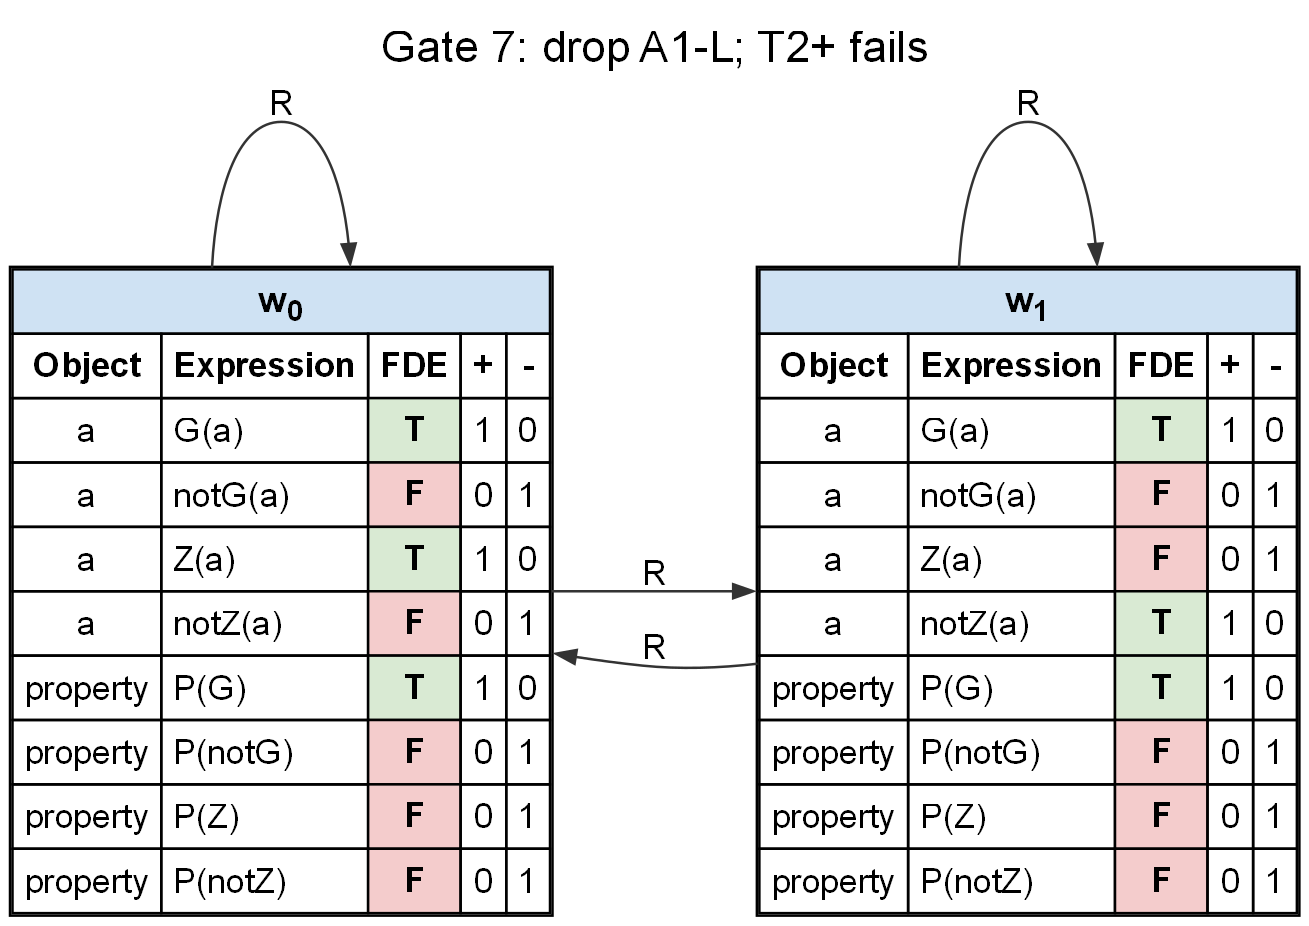
\includegraphics[width=0.96\linewidth]{figures/gate7_drop_a1_l_countermodel.png}
  \caption{The first Gate-7 \(T2^+\) countermodel found when only \(A1_L\) is dropped. The graph is generated by \texttt{formal/finite/visualize\_gate7\_models.py} from the same matrix family used in the 873-model exhaustive regression.}
  \label{fig:gate7-a1l-countermodel}
\end{figure}

The checker also verifies the schema-level equivalence
\[
  \MCp\leftrightarrow\MCm
\]
on a negation-closed two-world test family. The equivalence concerns schemata closed under substitution by negation, not a pointwise identity for one isolated formula valuation.

Gate 8 adds comparative witnesses. The support/exact comparison confirms that both Gate-6 T2 countermodels are support-Godlike but fail project-internal exact positive Godlikeness, while a separate exact-Godlike fixture still permits genuine \(\Both\) gluts. A complete-S5 bilateral Anderson fixture has positive necessary Godlike existence while a contingent formula application refutes positive modal collapse. Separate Scott and Anderson S4-style two-world models are reflexive and transitive but not symmetric and refute the corresponding reduced T3 conclusions.

The Fitting branch adds two further finite witnesses. First, a three-world two-entity model uses a selected negation-closed extensional property domain and satisfies the admissible Fitting recovery stack. At the root world the current frozen \(G\)-extension is both possibly and necessarily actually exemplified de re, and de-dicto Godlikeness is possible, but de-dicto necessary Godlikeness fails because the extension of \(G\) changes at another accessible world. The model therefore separates the two readings when the explicit extension-stability condition introduced below is absent.

Second, a complete two-world S5 model satisfies the encoded admissible Fitting stack, extension stability, and positive necessary actual Godlikeness. Its selected extension domain nevertheless contains genuine inconsistent information: one admissible extension takes value \(\Both\) on an entity, together with its FDE negation. A separate contingent intension \(Q\) satisfies
\[
  \pos{Q(a)}@w_0
\]
but not
\[
  \pos{\Box Q(a)}@w_0.
\]
Thus the present admissible bilateral Fitting candidate has an explicit necessary-God / no-positive-collapse model. This is a finite countermodel to collapse for the candidate, not an unbounded theorem about every Fitting semantics.

\subsection{Lean layer}
\label{sec:lean-layer}

The Lean package is pinned to Lean 4.30.0. It formalizes the four-valued carrier, FDE negation, conjunction and disjunction, bilateral relational modality, bilateral actualist quantification, signed necessary entailment, support-based Godlikeness, bilateral essence, and necessary-existence interfaces.

Lean proves the collapse-channel theorem generally at schema level and the Gate-5 truth-only possibility theorem
\[
  A1_R+A2^+\Longrightarrow T1_T.
\]
The principal Gate-6 Scott recovery theorem is machine-checked without a finite bound:
\[
  NegExemplification
  +G\text{-sup}
  +A1_L
  +R^+
  +REG_G
  \Longrightarrow T2^+.
\]

Gate 8 sharpens the later modal dependency. Once Scott \(T2^+\) is available, Lean proves
\[
  \operatorname{Sym}(R)
  +PossibleGod
  +T2^+
  +A5^+
  +NE\text{-sup}
  +G\text{-sup}
  \Longrightarrow T3^+.
\]
Reflexivity and transitivity are absent. Reflexivity enters only in the separate implication \(T3^+\Rightarrow GW\) and in the current essence-compressed collapse theorem
\[
  \operatorname{Refl}(R)
  +T2^+
  +T3^+
  +G\text{-sup}
  +CONST
  \Longrightarrow\MCp.
\]

For project-internal exact positive Godlikeness, Lean proves
\[
  G\text{-exact}^+\Rightarrow G\text{-sup}^+
\]
and
\[
  G\text{-exact}^+ + R^+\Longrightarrow T2_{\mathrm{exact}}^+.
\]
For Anderson, the literature-grounded positive interfaces and project-specific bilateral negative evidence are mechanized separately. Under classical coherence the negative necessary-exemplification, Godlikeness, essence, necessary-actual-exemplification, and necessary-existence clauses recover the complements of their positive counterparts. The positive Anderson necessary-existence branch reduces to symmetry alone:
\[
\begin{split}
  &\operatorname{Sym}(R)
  +PossibleG_A
  +G_A\text{-realization}
  +P^+(G_A)
  +A2^+\\
  &\qquad
  +NE_A\text{-realization}
  +P^+(NE_A)
  \Longrightarrow T3_A^+.
\end{split}
\]

\subsection{Classical recovery and verification discipline}
\label{sec:verification-discipline}

The Scott, Anderson, and admissible Fitting branches each have explicit recovery interfaces rather than relying on an informal assertion that the bilateral semantics ``becomes classical.'' Exact higher-order correspondence with the complete AFP/HOL developments is nevertheless a separate publication audit item.

The repository treats a countermodel or an obstruction theorem as a result rather than as a failed proof attempt. The unrestricted Fitting-comprehension obstruction is a particularly useful example: a theorem initially looked stronger because it lacked \(R^+\), but mechanization plus domain analysis revealed that the unrestricted regularity package excluded its intended witnesses. The admissible-domain reconstruction makes the subsequent theorem non-vacuous and is independently checked by finite models.

The explicit actualist quotient adds a third consistency check between the abstract and bounded layers. Lean's \texttt{FittingActualistQuotient.lean} constructs quotient entities, proves bilateral extension push/pull round trips, characterizes existence factorization, and identifies quotient entailment with ordinary entailment on pullbacks. The matching finite fixture exhausts all sixteen bilateral extensions in a two-entity one-class model and compares all 256 ordered entailment pairs. It also checks that \(\Both\) and \(\Neither\) survive quotienting and that split actual existence blocks representative-independent quotient interpretation.

The filter follow-up is split in the same way. The Lean quotient-filter module proves abstractly that point evaluation is a prime truth-order delta-filter which designates \(\Both\) but is not complement-deciding because of \(\Neither\). The finite oracle enumerates all filter families on the sixteen-element two-point quotient algebra and separately checks the non-adjunctive two-filter condition and a non-vacuous \(COMP\)-failure fixture.

The deferred paired-neighborhood layer now has the same two-sided validation. Lean proves modal duality, exact relational representation, and complement-dual classical recovery for arbitrary world types. The finite regression exhausts all \(256\) local two-world pairs of neighborhood families and all \(1024\) relational operator comparisons. The complete Python regression suite currently contains 31 tests.

All executable and Lean sources are maintained under \texttt{formal/}, with CI configured to run both tracks. General claims are promoted to machine-checked status only after an unbounded Lean theorem is present, while finite witnesses are reported as finite witnesses with their model bounds explicit. Appendix~\ref{sec:correspondence} maps every claim of the form ``Lean proves \(\dots\)'' in this manuscript to the named declaration that discharges it, and every bounded count to the fixture that produces it. Where the text abbreviates a premise list as a ``stack'', the Lean signature listed there is the authoritative statement.

\subsection{Fitting assumption minimization}
\label{sec:fitting-minimality}

The admissible-domain reconstruction permits a second round of dependency analysis. The original recovery package
\[
  REG_{G,F}^{adm}
  =COMP_{P,F}^{G,adm}+CONS_{G,F}^{G,adm}
\]
requires every admissible extension positively possessed by a positive Fitting-Godlike witness to be locally non-glutty. The proof of the extensional essence theorem, however, uses this consistency information only when positivity completeness classifies the possessed extension negatively. I therefore isolate the weaker condition
\[
\begin{split}
  NegCons_{G,F}^{adm}:\quad
  &Adm(Y)\land G_F^+(x,w)\land \pos{Y(x)}\land \neginfo{P(Y)}@w\\
  &\qquad\Longrightarrow \neg\neginfo{Y(x)}.
\end{split}
\]
Writing
\[
  REG_{G,F}^{neg}
  :=COMP_{P,F}^{G,adm}+NegCons_{G,F}^{adm},
\]
Lean proves
\[
  CONS_{G,F}^{G,adm}\Longrightarrow NegCons_{G,F}^{adm}
\]
and the strengthened recovery theorem
\[
\begin{split}
  &G\text{-admissible}
  +G_F\text{-realization}
  +A1_{L,F}^{adm}
  +REG_{G,F}^{neg}\\
  &\qquad\Longrightarrow
  G_F^+(x,w)\Rightarrow Ess_F^+(ext_wG,x,w).
\end{split}
\]
The corresponding de-re necessary-existence chain is machine-checked with the same targeted package. A one-world one-entity finite model separates the two consistency notions on the A1-L-only route: the sole admissible extension is genuinely glutty, the targeted negative-classification condition holds, full relevant exemplification consistency fails, and the realized positive Godlike extension is nevertheless an essence.

This weakening is itself directional. If the right A1 channel is restored, Lean proves
\[
  A1_{R,F}^{adm}
  +COMP_{P,F}^{G,adm}
  +NegCons_{G,F}^{adm}
  \Longrightarrow
  CONS_{G,F}^{G,adm}.
\]
Thus the reduction is not an unconditional weakening of a theory retaining both A1 directions. It instead exposes another division of labor between the two signed A1 flows: the A1-L recovery argument needs consistency only on the negative-classification branch, while A1-R supplies enough additional complement information to reconstruct the stronger consistency condition.

A separate minimization concerns de-dicto stability. Full bilateral extension stability
\[
  STAB_G^{\pm}:\qquad
  wRz\Rightarrow ext_wG\equiv ext_zG
\]
contains more information than the positive theorem uses. I split the positive channel into persistence and reflection:
\[
\begin{array}{rcl}
  Pers_G^+&:&wRz\land \pos{ext_wG(x)}\Rightarrow\pos{ext_zG(x)},\\
  Refl_G^+&:&wRz\land \pos{ext_zG(x)}\Rightarrow\pos{ext_wG(x)}.
\end{array}
\]
Their conjunction is written \(STAB_G^+\). Lean proves that bilateral stability implies \(STAB_G^+\), but the two positive directions are exactly what the de-dicto proof consumes: reflection converts de-dicto possibility into frozen de-re possibility, whereas persistence converts frozen de-re necessity back into de-dicto necessity. Consequently the minimized theorem is
\[
\begin{split}
  &G\text{-admissible}
  +G_F\text{-realization}
  +A1_{L,F}^{adm}
  +REG_{G,F}^{neg}\\
  &+NE_F\text{-realization}
  +A5_F^+
  +STAB_G^+
  +\Diamond^+\exists^E x\,G_F(x)\\
  &\qquad\Longrightarrow
  \Box^+\exists^E x\,G_F(x).
\end{split}
\]
No negative-extension stability and no S4/S5 frame condition occurs.

The weakening of stability is strict even under a stronger surrounding control theory. A complete two-world S5 fixture satisfies both A1 directions and the original full admissible regularity package. The positive membership set of \(G\) is \(\{a\}\) at both worlds, but negative information about a non-Godlike individual changes from falsity support to a gap. Hence \(STAB_G^+\) holds while \(STAB_G^{\pm}\) fails, and positive necessary de-dicto Godlikeness still holds. This finite witness shows that the positive theorem is genuinely insensitive to drift confined to the negative extension channel.

These results do not establish global minimality. They instead replace two coarse assumptions by proof-relevant interfaces and reveal a further interaction between the A1 split and the Fitting intension/extension architecture.

\input{sections/08b_fitting_domain_algebra}
\subsection{Entailment and the profile quotient}
\label{sec:fitting-entailment-quotient}

The preceding quotient construction raises a natural question: can the profile-saturation condition itself be generated by closing the admissible property domain under Fitting-style extensional entailment? The classical comparison suggests caution. In the mechanized Fitting analysis, the \(\delta\)-filter is a family of positive extensions: it contains the universal extension, excludes the empty extension, is upward closed under supersets, and is closed under intersections \cite{BenzmuellerFuenmayor2019}. This is closure of the positivity filter, not closure of the ambient property domain. The present \(A2_F^+\) interface already captures the corresponding monotonicity of positive support under extensional entailment.

I therefore distinguish that source-grounded filter behavior from the stronger domain principle
\[
\begin{split}
  EntCl^{adm}:\quad
  &Adm(X)\land
  \forall w\,Entail_F^+(w,X,Y)\\
  &\qquad\Longrightarrow Adm(Y).
\end{split}
\]
The stronger principle is unsuitable once FDE bottom is admitted. Since \(\bot_F\) has no positive members,
\[
  Entail_F^+(w,\bot_F,Y)
\]
holds vacuously for every world \(w\) and every rigid extension \(Y\). Lean consequently proves
\[
\boxed{
  EntCl^{adm}+Adm(\bot_F)
  \Longrightarrow
  \forall Y\,Adm(Y).
}
\]
Thus naive entailment closure of the admissible property universe reconstructs unrestricted bilateral comprehension. Combined with relevant exemplification consistency, the earlier comprehension obstruction returns immediately:
\[
\boxed{
  EntCl^{adm}+Adm(\bot_F)+CONS_{G,F}^{G,adm}
  \Longrightarrow
  \forall w,x\;\neg G_F^+(x,w).
}
\]
The distinction between filter closure and domain closure is therefore substantive rather than terminological.

A finite separation strengthens this negative result. Over two entities I take the complete \(4^2=16\) bilateral extension universe as admissible. Both entities actually exist at one reflexive world, and positive support is assigned exactly to extensions whose positive channel contains both entities. This model satisfies \(A2_F^+\), full domain-level entailment closure, closure under the basic FDE extension algebra, and quotient-compatible actual existence. Positivity nevertheless gives the two entities the same positive-property profile while an admissible singleton extension distinguishes them. Hence
\[
\boxed{
  A2_F^+
  +EntCl^{adm}
  +\text{FDE algebra closure}
  +\text{profile-compatible existence}
  \not\Longrightarrow Sat_P^{adm}
}
\]
in this explicit finite model. Entailment closure therefore does not generate the missing quotient structure.

The positive result takes a different form. For each world \(w\), define a bilateral profile closure on arbitrary rigid extensions by
\[
\begin{aligned}
  +Sat_w(Y)(x)
  &\Longleftrightarrow
  \exists y\,(x\approx_w^+y\land +Y(y)),\\
  -Sat_w(Y)(x)
  &\Longleftrightarrow
  \exists y\,(x\approx_w^+y\land -Y(y)).
\end{aligned}
\]
Lean proves that \(Sat_w\) is extensive and monotone and is idempotent up to bilateral extensional equivalence. Every \(Sat_w(Y)\) respects the positive-profile quotient. More strongly, if \(Z\) already respects the quotient and \(Y\) is support-included in \(Z\), then
\[
  Sat_w(Y)\preceq Z.
\]
Thus \(Sat_w(Y)\) is the least quotient-respecting bilateral extension above \(Y\) in the support-inclusion order.

This yields an exact fixed-point characterization of the earlier domain condition:
\[
\boxed{
  Sat_P^{adm}
  \Longleftrightarrow
  \forall w,Y\,
  \bigl(Adm(Y)\rightarrow Sat_w(Y)\equiv Y\bigr).
}
\]
The quotient route can therefore be read as selecting admissible properties from the fixed points of a canonical closure operator induced by positive-property observational equivalence.

Actualist quantification introduces one further boundary. Fitting entailment quantifies only over entities that actually exist at accessible worlds. Even if two entities lie in the same positive-profile class, the existence predicate can still distinguish them. I isolate the compatibility condition
\[
\begin{split}
  ExSat_P:\quad
  wRz\land x\approx_w^+y
  \Longrightarrow
  \bigl(E(z,x)\leftrightarrow E(z,y)\bigr).
\end{split}
\]
Under this premise Lean proves
\[
\boxed{
  Entail_F^+(w,X,Y)
  \Longrightarrow
  Entail_F^+(w,Sat_w(X),Sat_w(Y)).
}
\]
Hence actualist Fitting entailment descends through the profile closure when actual existence itself factors through the same quotient.

A second finite fixture shows why the existence premise matters. Two entities have the same positive-property profile, but at the sole accessible target world only one actually exists. An extension whose only positive member is the non-actual representative then entails an empty-positive extension vacuously. Profile closure transfers that positive membership to the equivalent actual representative, after which the saturated entailment fails. Thus the existence-compatibility condition is not merely a notational convenience, although the finite witness does not establish its global necessity for every alternative quotient construction.

The resulting architecture is more precise than the initial entailment-closure hypothesis. Positivity-filter closure remains governed by \(A2_F^+\); the admissible property universe should not be closed indiscriminately under entailment; profile saturation is instead a fixed-point condition for a canonical closure operator; and actualist entailment is compatible with that quotient only when actual existence respects the relevant profile classes. This relocates the next open problem from property-domain entailment closure to the principled status of the actualist quotient condition and to the algebraic/filter structure of the closure fixed points.

\section{Related Work}
\label{sec:related}

The project sits at the intersection of two mature lines of work whose combination motivates the present question. First, G\"odel--Scott and related ontological theories have been extensively reconstructed and analyzed with computational tools, including comparisons of Scott, Anderson, and Fitting variants and their behavior with respect to modal collapse \cite{BenzmuellerScott2025,BenzmuellerFuenmayor2019}. Recent machine-checked analysis further separates positivity rigidity from ultrafilter structure as explanations of collapse \cite{Benzmueller2026Collapse}.

The Anderson/Fitting comparison is especially relevant to Gate 8. The computer-supported analysis of Benzm\"uller and Fuenmayor distinguishes intensional properties from their extensions and shows that this distinction is central to comparing the two non-collapsing variants \cite{BenzmuellerFuenmayor2019}. In the source IHOML treatment, Scott and Anderson apply positivity to intensional properties, whereas Fitting moves the positivity predicate to property extensions. The present project therefore does not model Fitting by merely changing axioms over the existing single property type. Instead, the first Fitting milestone introduces distinct Lean types for bilateral extensions and world-indexed intensions before any Fitting essence or necessary-existence theorem is attempted.

The same literature also motivates a methodological distinction in the Anderson branch. Anderson strengthens Godlikeness by classifying the necessary properties of an individual through positivity and modifies essence accordingly, rather than merely adding a stronger Scott-style reflection principle \cite{BenzmuellerFuenmayor2019}. The bilateral negative clauses used here are consequently a project-specific FDE reconstruction around a literature-grounded positive interface; they are not attributed to Anderson himself.

Second, Belnap--Dunn/FDE semantics provides the canonical four-valued distinction between truth-only, falsity-only, both, and neither \cite{Belnap1977,Dunn1976}. Modal extensions with Belnapian values have been developed using Kripke and algebraic semantics \cite{OdintsovWansing2010,RivieccioJungJansana2017}. Particularly close in semantic neighborhood is Petrukhin's recent treatment of essence and accident modalities in an S5-based four-valued setting \cite{Petrukhin2026}.

\paragraph{Novelty status.}
A dedicated prior-art review specifically targeting four-valued or FDE-based reconstructions of the G\"odel--Scott positivity axioms, Anderson-style necessary-property definitions, and Fitting-style extensional positivity remains required before any novelty claim is made. The manuscript therefore states structural and mechanization results only. In particular, the symmetry-only T3 reductions, the bilateral Anderson candidate, and the Fitting type split are project results whose relation to all prior non-classical reconstructions still requires the Gate-9 audit.

\section{Conclusion and Research Agenda}
\label{sec:conclusion}

This manuscript treats the G\"odel--Scott theory not merely as an object to be translated from two values to four, but as a controlled test case for locating informational dependencies that classical bivalence suppresses.

By version 0.7 the main reconstruction and verification branches have both reached positive necessary God-like existence and the associated collapse analysis. Gates 1--4 establish the bilateral propositional and modal semantics, decompose A1 and A4, falsify the original collapse-separation conjecture under involutive FDE negation, and isolate glut/gap failures in the classical reflection step. Gate 5 reconstructs truth-only positive-property exemplification, a control reading of A3, possible positive God-like existence, and support-based bilateral Godlikeness.

Gate 6 identifies the sharper bottleneck. A natural bilateral definition of essence recovers Scott D2 classically, but it does not make Godlikeness an essence automatically. Two explicit two-world S5 models satisfy the Gate-5 control conditions together with strong A1 and positive rigidity while refuting
\[
  T2^+:\quad
  \pos{G(x)}\Rightarrow\pos{G\operatorname{Ess}x}.
\]
The models fail for different reasons. In the glut model a locally possessed property is also negatively supported and need not be positively shared by another God-like witness. In the gap model positivity supplies no information capable of turning local possession into necessary sharing.

A targeted regularity package recovers T2. For properties positively exemplified by positive God-like witnesses, relevant positivity completeness blocks the gap route while relevant exemplification consistency blocks the glut route. Together with \(A1_L\), positive rigidity, support-based Godlikeness, and the bilateral negation law these conditions yield positive Godlikeness-as-essence.

Gate 7 changes the epistemic status of this result. Lean 4.30.0 machine-checks the general implication
\[
  NegExemplification
  +G\text{-sup}
  +A1_L
  +R^+
  +REG_G
  \Longrightarrow T2^+.
\]
The earlier truth-only possibility theorem is also machine-checked:
\[
  A1_R+A2^+\Longrightarrow T1_T.
\]
Thus the division of labor inside Scott's A1 is not only semantically motivated but represented in independent formal derivations.

Once T2 is available, the remaining necessary-existence branch is considerably more robust. Lean verifies that possible positive Godlikeness together with \(T2^+\), \(A5^+\), the positive necessary-existence realization, support-based Godlikeness, and S5 yields
\[
  T3^+:\quad \pos{\Box\exists^E x\,G(x)}.
\]
On reflexive frames, T3 supplies the global witness condition \(GW\). Lean also verifies the essence-compressed positive collapse theorem: positive T2, positive T3, support-based Godlikeness, and constant-property embedding entail positive modal collapse. The informative negative collapse schema then follows from the separately machine-checked collapse-channel equivalence under involutive FDE negation.

The finite-model layer provides the complementary negative evidence. It regression-checks the T1 positivity-glut obstruction and both T2 countermodels. A broader exhaustive two-world, one-entity \(G,Z\) family retains 873 models satisfying \(A1_L\), positive rigidity, relevant positivity completeness, and relevant exemplification consistency together with the fixed bilateral semantic laws. Every retained model satisfies \(T2^+\). Dropping any one of those four recovery assumptions individually yields a T2 countermodel in that same bounded family.

This bounded result sharpens but does not settle the minimality question. It establishes individual indispensability relative to a specific complete finite family, not global model-theoretic necessity. The principal open problem is therefore now explicitly:
\[
  \boxed{
  \text{Which weaker principled four-valued assumptions, if any, suffice for }T2^+\text{ globally?}
  }
\]

Classical recovery has also been formalized at the bilateral interfaces. Under explicit classical coherence, negative support for necessary entailment, Godlikeness, essence, and necessary existence is exactly the complement of the corresponding positive support. This supports the intended reduction to ordinary bivalent behavior without claiming that the full AFP/HOL Scott development has already been reproduced line by line.

The next phase should therefore compare theories rather than continue altering the S5 control semantics. The immediate targets are `G-sup` versus `G-exact`, selected Anderson/Fitting-style variants, weaker modal frame conditions, and later the paired-neighborhood generalization. Exact higher-order correspondence with the frozen Scott baseline and the dedicated prior-art audit remain publication-stage requirements.

The paper continues to distinguish general semantic theorems, machine-checked results, finite countermodels, bounded exhaustive evidence, and open global-minimality claims explicitly.


\bibliographystyle{plain}
\bibliography{references}
\end{document}
